% sections/system.tex: Section 2, the system (what the tool does, how a creator uses it, design principles).
% Draft 2, 2026-10-24: cut from about 1,140 to about 640 words to fit 4 pages (notes/CUTS.md).
% CE = ../citation-equity (the tool repo, read only). Every number carries a "% src:" comment.
% Labels defined here: sec:system, sec:checks, sec:suggest, sec:beyond, sec:bench, fig:workspace.

\section{Citation Equity}\label{sec:system}

% src (CE c908431): CE/README.md lines 11 to 23 ("What it does", "How to use it"); up to eight: CE/apps/workspace/lib/questions.ts
%      line 12 (MAX_QUESTIONS = 8); CE/docs/superpowers/specs/2026-10-23-citation-equity-design.md sections 1 and 4 (local feat
%      branch only; not on public main b10887e)
A writer pastes a draft, sets up to eight target questions, applies fixes one at a time and tests the revision.
% src: CE/README.md line 68 ("Privacy": the CLI sends the draft only to "a hosted API you choose") and CE/docs/cli.md line 89
%      ("Drafts stay on your disk unless you point `ce bench` at a hosted server"); beside, never inside: CE/docs/architecture.md
%      line 27 ("It reports; it never retunes the weights.") and CE/docs/evidence.md line 14 ("reports a measured outcome
%      separately from the score"), CE c908431
Measured outcomes are reported beside the score, never inside it, and drafts stay local unless the author picks a hosted model.
% src (CE c908431): CE/docs/architecture.md lines 3 to 18 (monorepo, no server), 34 (engine: browser and CLI), 49 to 59 (bench),
%      67 (static export, GitHub Pages) and 104 (Playwright: "no request leaving the origin on load")
A TypeScript monorepo holds an \emph{engine} of pure check functions (browser and CLI), a \emph{bench} with the citation test, and a \emph{workspace}, a Next.js static export on GitHub Pages with no server; a browser test asserts no request leaves the origin on load.
% src: data/system_checks.json (scripts/system_checks.py, rerun 2026-10-26 at CE c908431, tree clean): analyze() median 7.47 ms
%      (espresso, 831 words) and 10.21 ms (RAG, 1,041 words), 60 warm runs, Apple M4 Pro; three reruns of scripts/engine_time.mts
%      gave 10.6 to 11.0 ms for RAG; /draft/ loads 801,485 B of gzipped JS; 1,248 Vitest tests passed; 78 Playwright tests
%      (each spec against the root and the GitHub Pages build). The earlier 6 ms and 1,171 were measured at CE 2851854,
%      before the reader's-words check existed.
The engine checks a 1{,}000-word draft in about 10\,ms on a laptop; 1{,}248 unit and 78 browser tests cover the code.

\subsection{Check: eleven checks with graded evidence}\label{sec:checks}

% src (CE c908431): CE/docs/evidence.md line 3 (six from Prof. Bayat's design for the project, i.e. the PI's; four from the
%      literature; one, your reader's words up top, added because it helped in E1); CE/docs/architecture.md line 30;
%      CE/packages/engine/src/registry.ts lines 13 to 17
Six checks come from the project's initial design, four from the literature (Figure~\ref{fig:evidence} names them all), and one, \emph{your reader's words up top}, from our own test, where it helped (Section~\ref{sec:findings});
% src: CE/README.md lines 21 ("Not scored") and 27 ("seven are averaged into the AI-ready score"); CE/docs/evidence.md line 34; CE/docs/architecture.md line 30 (weight 0 in both built-in
%      weightings, still analyzed and still suggest); CE/packages/engine/src/registry.ts lines 98 to 128 (UNSCORED_CHECKS,
%      PRESET_WEIGHTS); owner approved the change (task brief, 2026-10-24)
four (question headings, lists, cited sources, direct answer first) are shown and still suggest fixes but are not scored, as our tests found no clear effect on citation.
% src: CE/docs/evidence.md lines 16 to 32 (rubric; the null rule at lines 24 and 29) and line 34 (outcome); lines 76 to 88 ("The
%      studies", the nine sources), CE c908431
Each check scores the draft from 0 to 1 and carries an evidence grade (strong, moderate, mixed or untested) under a written rubric in which a null or negative result in any study, even in one subgroup, makes a check mixed.
% src: CE/docs/evidence.md line 3 ("opened and read on 2026-10-23") and line 34 ("Nine are mixed and two are untested");
%      "in full" dropped (verify-claims B6)
% The nine sources are cited in Figure 3's caption, in column order (clarity pass 2026-10-26).
Over the nine sources the tool cites, each opened and read, no check is strong or moderate: nine are mixed and two untested (Figure~\ref{fig:evidence}).
% src: data/evidence_grades_loose.json (scripts/derive_loose_grades.py): loose rule 0 strong, 5 moderate, 4 mixed, 2 untested
%      (lists, direct-answer lead, question coverage, comparisons and reader's words move to moderate); single-rater coding,
%      the reader's-words cells coded 2026-10-24 (notes/FINAL-TOOL-SYNC.md)
A looser rule, defined post hoc, that counts only a study's own no-effect conclusion or a significant harm makes five mixed checks moderate. \owner{Second rater (Ishan Gupta): agreement pending.}
% src: CE/README.md lines 27 and 32; CE/packages/engine/src/registry.ts lines 98 to 128; CE/apps/workspace/components/draft/score-card.tsx
%      line 112 (shipped wording "A writing checklist, not a forecast."; CE/apps/workspace/lib/presets.ts lines 11 to 12 keep
%      "not a prediction of citations" for the weighting notes).
% src: UI name "AI-ready score": CE/README.md lines 11 and 27, CE/docs/architecture.md line 39 and CE/docs/evidence.md line 7
%      ("The AI-ready score is a content check"), CE c908431; Figure 2 shows "AI-ready score".
The \emph{checklist score} (the tool's AI-ready score) averages the checks out of 100 under editable weights and is labelled a writing checklist, not a forecast.

\subsection{Suggest, never rewrite}\label{sec:suggest}

% src (CE c908431): CE/docs/architecture.md lines 26 (anchored ranges), 78 (anchors follow the author's edits; merge preview),
%      81 (CE/apps/workspace/lib/apply.ts: Apply only if the text is unchanged, else "Out of date"; "There is no bulk action."),
%      84 (Rewrite with local AI only after a click) and 104 (Preview, Apply, Undo, Done, Skip); CE/README.md line 13;
%      side by side: CE/apps/workspace/components/draft/draft-view.tsx lines 683 to 686 ("opens the proposal side by side.
%      Nothing is applied here.")
% src: AnchoredAI arXiv 2509.16128: within-subjects lab study, more agency and ownership than a chat interface
Comments anchored to spans of text improved writers' agency over a chat interface in a lab study~\cite{lou2025anchoredai}, so every suggestion is anchored to an exact range of the draft and follows the author's own edits.
An \emph{edit} (say, a missing question mark) is previewed, and Apply changes the range only if its text is unchanged; an \emph{advisory} (say, name a real source for a figure) is left to the author.
Every action has Undo, and there is no ``apply all'' (Figure~\ref{fig:workspace}). An optional local model can propose wording for one suggestion, shown side by side and applied only on the author's click.
% "Beyond the draft" was a \paragraph; the clarity pass (2026-10-26) runs it on in this paragraph (notes/CUTS.md 79).
% src (CE c908431): CE/README.md line 15; CE/docs/architecture.md lines 44 (seven readiness items) and 74 (/cited/: cited sites
%      grouped by type); CE/docs/evidence.md line 262 ("no readiness item changes a score"), lines 264 to 271 (readiness rubric:
%      operator documentation counts) and the grades at lines 277, 289, 301, 315, 328, 338, 372 (2 strong, 1 moderate, 2 mixed,
%      2 untested)
\emph{Beyond the draft}, \emph{site readiness}\label{sec:beyond} checks seven items of the published page (crawler access and indexing directives are graded strong, on operators' documentation); % src: CE/README.md (Your questions; Searches behind this question), CE 96375d4; CE/docs/cli.md (ce questions --keywords --fanout)
\emph{who gets cited} sorts the sources of pasted AI answers; \emph{your questions} turns keywords or Search Console queries into a ranked list of reader questions for the whole site, each with the searches an answer engine is likely to run behind it. None changes the score, and the last two are untested helpers.

\subsection{Test it: the citation bench}\label{sec:bench}

% src (CE c908431): CE/samples/README.md line 39 ("How the test works") and line 81 (settings); CE/docs/architecture.md lines 52
%      (BM25, top k = 8), 54 (N = 8 seeds, seeded shuffle of the source order), 55 (chance level, exact sign-flip test) and 63
%      ("It does not predict live AI engines."); valid answers and failures: CE/samples/README.md line 56
% src: Martinez arXiv 2607.14035 Section 11.2 (randomized context order; "Seven to eight repetitions"; failed outputs are outcomes)
% src: "plus one format reminder": CE/samples/README.md line 55 (GEO's instruction word for word, one line added after the sources)
For each question, BM25 retrieves the top 8 of the draft and its competitor pages, and a model the author runs (\texttt{llama3.2:3b} through Ollama by default) answers with numbered citations under GEO's prompt plus one format reminder~\cite{aggarwal2024geo}, 8 times with different seeds and source orders~\cite[Sec.~11.2]{martinez2026survey}.
Reports keep apart how often the draft was retrieved, how many answers were \emph{valid} (failures are outcomes, not discarded data), how often it was cited, and its \emph{word share} beside the \emph{chance level} of an even split (0.125), with a paired sign-flip test; each says \emph{``It does not predict live AI engines.''}
% src: CE/samples/README.md line 83 (espresso 18:37 to 18:52, RAG 18:52 to 19:10 PDT: 64 answers per sample, 2 drafts x 4
%      questions x 8 runs, in 15 and 18 min: 14.1 and 16.9 s per answer) and line 82 (Apple M4 Pro, 24 GB, Ollama 0.40.9);
%      CE/docs/cli.md line 73 (`ce bench --export-prompts` and `--answers`: export, then replay answers generated elsewhere)
% Clarity pass 2026-10-26 (notes/CUTS.md 79): "An answer takes 14 to 17 s on the authors' laptop;" dropped; Section 5 keeps
% the live run's 64 answers in 15 minutes (same README line 83).
For larger models it exports the prompts and replays answers generated elsewhere.
% src: CE/samples/README.md line 98 ("With 4 questions the smallest possible p is 0.125, so these runs can show a direction at most.")
% Cut 2026-10-26 (notes/CUTS.md 72): "With a sample's 4 questions the smallest possible p is 0.125, so a laptop run shows a
% direction at most." The p floor moved into Section 3's laptop paragraph.

\begin{figure}[t]
  \centering
  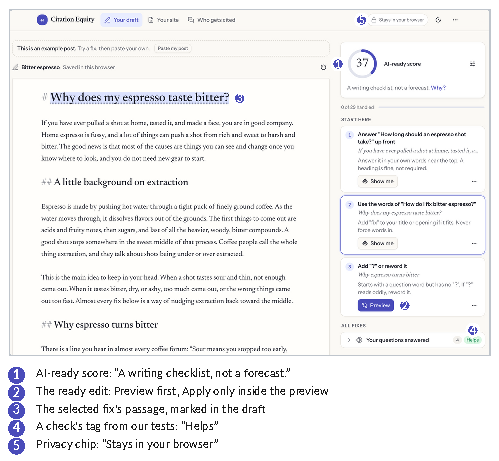
\includegraphics[width=\columnwidth]{figures/fig2_workspace.pdf}
  \Description{A screenshot of the workspace's draft view on the espresso example. Left: the draft as a paper-style page, with its title underlined because the selected tip is about it. Right: the AI-ready score of 37 with the line "A writing checklist, not a forecast", three Start-here fixes (two tips and one ready edit with a Preview button), and the first fix group with the tag "Helps". Top right: a "Stays in your browser" chip. Numbered callouts point to each.}
  % takeaway rewritten 2026-10-26: since CE 008e68e the draft view shows no grades; a fix group carries at most one chip,
  % "Helps" or "Not scored" (CE/apps/workspace/components/check-chip.tsx; CE/README.md line 21); grades live on /research.
  \caption{\figtakeaway{The deployed draft view (espresso example): the author applies one fix at a time; a tag marks the checks our tests found to help.}}
  \label{fig:workspace}
\end{figure}
